\chapter{Bayesian model average}\label{chap10}

\section{Solutions of Exercises}\label{sec101}
\begin{enumerate}[leftmargin=*]

	\item The Gaussian linear model specifies $\bf{y}=\alpha\bm{i}_N+\bm{X}_m\bm{\beta}_m+\bm{\mu}_m$ such that $\bm{\mu}_m\sim{N}(\bm{0},\sigma^2\bm{I}_n)$, and $\bm{X}_m$ does not have the column of ones. Assuming that $\pi(\sigma^2)\propto 1/{\sigma^2}$, $\pi(\alpha)\propto 1$, and $\bm{\beta}_m|\sigma^2 \sim {N}(\bm{0}_{k_m}, \sigma^2 (g_m\bm{X}_m^{\top}\bm{X}_m)^{-1})$.
\begin{itemize}
	\item Show that the conditional posterior distribution of $\bm{\beta}_m$ is $N(\bm{\beta}_{mn},\sigma^2\bm{B}_{mn})$, where $\bm{\beta}_{mn}=\bm{B}_{mn}\bm{X}_m^{\top}\bm{y}$ and $\bm{B}_{mn}=((1+g_m)\bm{X}_m^{\top}\bm{X}_m)^{-1}$.
	\item Show that the marginal the marginal likelihood associated with model $\mathcal{M}_m$ is proportional to
	\begin{align*}
		p(\bm{y}|\mathcal{M}_m)&\propto \left(\frac{g_m}{1+g_m}\right)^{k_m/2} \left[(\bm{y}-\bar{y}\bm{i}_N)^{\top}(\bm{y}-\bar{y}\bm{i}_N)-\frac{1}{1+g_m}(\bm{y}^{\top}\bm{P}_{X_m}\bm{y})\right]^{-(N-1)/2},
	\end{align*}
	where all parameter are indexed to model $\mathcal{M}_m$, $\bm{P}_{X_m}=\bm{X}_m(\bm{X}_m^{\top}\bm{X}_m)^{-1}\bm{X}_m$ is the projection matrix on the space generated by the columns of $\bm{X}_m$, and $\bar{y}$ is the sample mean of $\bm{y}$.
	
	Hint: Take into account that $\bm{i}_N^{\top}\bm{X}_m=\bm{0}_{k_m}$ due to all columns being centered with respect to their means.
\end{itemize}
\textbf{Answer}

The marginal likelihood of this model is

\begin{align*}
	p({\bf{y}})&=\int_0^{\infty}\int_{R^K}\int_R\pi (\bm{\beta} | \sigma^2)\pi(\sigma^2)\pi(\alpha)p({\bf{y}}|\bm{\beta}, \sigma^2, \alpha)d\alpha d\bm{\beta} d\sigma^2\\
	&\propto \int_0^{\infty}\int_{R^K}\int_R (\sigma^2)^{-k_m/2} |g_m\bm{X}_m^{\top}\bm{X}_m|^{1/2}\exp\left\{-\frac{1}{2\sigma^2}(\bm{\beta}^{\top}(g_m\bm{X}_m^{\top}\bm{X}_m)\bm{\beta})\right\}(\sigma^2)^{-1}\\
	&\times (\sigma^2)^{-N/2}\exp\left\{-\frac{1}{2\sigma^2}(\bm{y}-\alpha\bm{i}_N-\bm{X}_m\bm{\beta})^{\top}(\bm{y}-\alpha\bm{i}_N-\bm{X}_m\bm{\beta})\right\}d\alpha d\bm{\beta} d\sigma^2.
\end{align*}
Taking into account that $(\bm{y}-\alpha\bm{i}_N-\bm{X}_m\bm{\beta})^{\top}(\bm{y}-\alpha\bm{i}_N-\bm{X}_m\bm{\beta})=(\bm{y}-\bm{X}_m\bm{\beta})^{\top}(\bm{y}-\bm{X}_m\bm{\beta})+N(\alpha-\bar{y})^2-N\bar{y}^2$, 

\begin{align*}
	p({\bf{y}})	&\propto \int_0^{\infty}\int_{R^K} (\sigma^2)^{-k_m/2} |g_m\bm{X}_m^{\top}\bm{X}_m|^{1/2}\exp\left\{-\frac{1}{2\sigma^2}(\bm{\beta}^{\top}(g_m\bm{X}_m^{\top}\bm{X}_m)\bm{\beta})\right\}(\sigma^2)^{-1}\\
	&\times (\sigma^2)^{-N/2}\exp\left\{-\frac{1}{2\sigma^2}[(\bm{y}-\bm{X}_m\bm{\beta})^{\top}(\bm{y}-\bm{X}_m\bm{\beta})-N\bar{y}^2]\right\}\\
	&\times \int_R \exp\left\{-\frac{1}{2\sigma^2}(N(\alpha-\bar{y})^2)\right\} d\alpha d\bm{\beta} d\sigma^2.
\end{align*}

The last term is the kernel of a normal density function with mean $\bar{y}$ and variance $\sigma^2/N$, then

\begin{align*}
	p({\bf{y}})	&\propto \int_0^{\infty}\int_{R^K} (\sigma^2)^{-k_m/2} |g_m\bm{X}_m^{\top}\bm{X}_m|^{1/2}\exp\left\{-\frac{1}{2\sigma^2}(\bm{\beta}^{\top}(g_m\bm{X}_m^{\top}\bm{X}_m)\bm{\beta})\right\}(\sigma^2)^{-1}\\
	&\times (\sigma^2)^{-N/2}(\sigma^2)^{1/2}\exp\left\{-\frac{1}{2\sigma^2}[(\bm{y}-\bm{X}_m\bm{\beta})^{\top}(\bm{y}-\bm{X}_m\bm{\beta})-N\bar{y}^2]\right\}d\bm{\beta} d\sigma^2.
\end{align*}

Collecting terms for $\bm{\beta}$, we have $(\bm{y}-\bm{X}_m\bm{\beta})^{\top}(\bm{y}-\bm{X}_m\bm{\beta})-N\bar{y}^2+\bm{\beta}^{\top}(g_m\bm{X}_m^{\top}\bm{X}_m)\bm{\beta}=(\bm{\beta}-\bm{\beta}_{mn})^{\top}\bm{B}_{mn}^{-1}(\bm{\beta}-\bm{\beta}_{mn})+\bm{y}^{\top}\bm{y}-N\bar{y}^2-\bm{\beta}_{mn}^{\top}\bm{B}_{mn}\bm{\beta}_{mn}$ where $\bm{\beta}_{mn}=\bm{B}_{mn}\bm{X}^{\top}\bm{y}$ and $\bm{B}_{mn}=((1+g_m)\bm{X}^{\top}\bm{X})^{-1}$. Then,

\begin{align*}
	p({\bf{y}})	&\propto \int_0^{\infty} (\sigma^2)^{-k_m/2} |g_m\bm{X}_m^{\top}\bm{X}_m|^{1/2}\exp\left\{-\frac{1}{2\sigma^2}(\bm{y}^{\top}\bm{y}-N\bar{y}^2-\bm{\beta}_{mn}^{\top}\bm{B}_{mn}\bm{\beta}_{mn})\right\}(\sigma^2)^{-1}\\
	&\times (\sigma^2)^{-N/2}(\sigma^2)^{1/2}\int_{R^K}\exp\left\{-\frac{1}{2\sigma^2}(\bm{\beta}-\bm{\beta}_{mn})^{\top}\bm{B}_{mn}^{-1}(\bm{\beta}-\bm{\beta}_{mn})\right\}d\bm{\beta} d\sigma^2.
\end{align*}
The last term is the kernel of a multivariate normal density with mean $\bm{\beta}_{mn}$ and variance $\bm{B}_{mn}$ (proof of the first bullet). Then,

\begin{align*}
	p({\bf{y}})	&\propto \int_0^{\infty}\left(\frac{g_m}{1+g_m}\right)^{k_m/2}(\sigma^2)^{-(N-1)/2-1} \exp\left\{-\frac{1}{2\sigma^2}(\bm{y}^{\top}\bm{y}-N\bar{y}^2-\bm{\beta}_{mn}^{\top}\bm{B}_{mn}\bm{\beta}_{mn})\right\}d\sigma^2.
\end{align*}

This is the kernel of an inverse-gamma density with parameters $\alpha_n=(N-1)/2$ and $\delta_n=\bm{y}^{\top}\bm{y}-N\bar{y}^2-\bm{\beta}_{mn}^{\top}\bm{B}_{mn}\bm{\beta}_{mn}$, where $\bm{y}^{\top}\bm{y}-N\bar{y}^2-\bm{\beta}_{mn}^{\top}\bm{B}_{mn}\bm{\beta}_{mn}=(\bm{y}-\bm{i}_N\alpha)^{\top}(\bm{y}-\bm{i}_N\alpha)-(1+g_m)^{-1}\bm{y}^{\top}(\bm{X}(\bm{X}^{\top}\bm{X})^{-1}\bm{X}^{\top})\bm{y}$. Then,

\begin{align*}
	p(\bm{y}|\mathcal{M}_m)&\propto \left(\frac{g_m}{1+g_m}\right)^{k_m/2} \left[(\bm{y}-\bar{y}\bm{i}_N)^{\top}(\bm{y}-\bar{y}\bm{i}_N)-\frac{1}{1+g_m}(\bm{y}^{\top}\bm{P}_{X_m}\bm{y})\right]^{-(N-1)/2},
\end{align*}

\item \textbf{Determinants of export diversification I}

\cite{Jetter2015} use BMA to study the determinants of export diversification. Use the dataset \textit{10ExportDiversificationHHI.csv} to perform BMA using the BIC approximation and MC3 with 10000 iterations to check if these two approaches agree.

\textbf{Answer}

The first aspect to note is that the BIC approximation is faster by far than the MC3 algorithm. We see from the results that the two approaches show that the most relevant variables to determine export diversification are \textit{avgedu5} (primary education) and \textit{avgnatres} (natural resources). See \cite{Jetter2015} for details of all variables. The model with the highest PMP using MC3 includes these two variables (PMP = 0.16), while the model with the highest PMP using the BIC approximation in addition to these two variables also includes Portugal former colony and population (PMP = 0.03). Both methods agree that export diversification increases with primary education, and decreases with natural resources.     

	\begin{tcolorbox}[enhanced,width=4.67in,center upper,
	fontupper=\large\bfseries,drop shadow southwest,sharp corners]
	\textit{R code. Determinants of export diversification}
	\begin{VF}
		\begin{lstlisting}[language=R]
rm(list = ls()); set.seed(010101)
Data <- read.csv("https://raw.githubusercontent.com/besmarter/BSTApp/refs/heads/master/DataApp/10ExportDiversificationHHI.csv", sep = ",", header = TRUE, quote = "")
attach(Data)
y <- Data[,1]; X <- as.matrix(Data[,-1]); K <- dim(X)[2]
BMAglm <- BMA::bicreg(X, y, strict = FALSE, OR = 50)
summary(BMAglm)
BMAreg <- BMA::MC3.REG(y, X, num.its=10000)
Models <- unique(BMAreg[["variables"]])
nModels <- dim(Models)[1]
nVistModels <- dim(BMAreg[["variables"]])[1]
PMPmc3 <- NULL
for(m in 1:nModels){
	idModm <- NULL
	for(j in 1:nVistModels){
		if(sum(Models[m,] == BMAreg[["variables"]][j,]) == K){
			idModm <- c(idModm, j)
		}else{
			idModm <- idModm
		} 
	}
	PMPm <- sum(BMAreg[["post.prob"]][idModm])
	PMPmc3 <- c(PMPmc3, PMPm)
}
PMPmc3
PIPmc3 <- NULL
for(k in 1:K){
	PIPk <- sum(PMPmc3[which(Models[,k] == 1)])
	PIPmc3 <- c(PIPmc3, PIPk)
}
plot(PIPmc3)
Meansmc3 <- matrix(0, nModels, K)
Varsmc3 <- matrix(0, nModels, K)
for(m in 1:nModels){
	idXs <- which(Models[m,] == 1)
	if(length(idXs) == 0){
		Regm <- lm(y ~ 1)
	}else{
		Xm <- X[, idXs]
		Regm <- lm(y ~ Xm)
		SumRegm <- summary(Regm)
		Meansmc3[m, idXs] <- SumRegm[["coefficients"]][-1,1]
		Varsmc3[m, idXs] <- SumRegm[["coefficients"]][-1,2]^2 
	}
}
BMAmeansmc3 <- colSums(Meansmc3*PMPmc3)
BMAsdmc3 <- (colSums(PMPmc3*Varsmc3)  + colSums(PMPmc3*(Meansmc3-matrix(rep(BMAmeansmc3, each = nModels), nModels, K))^2))^0.5 
plot(BMAmeansmc3)
plot(BMAsdmc3)
Ratio <- BMAmeansmc3/BMAsdmc3
RessulMC3 <- as.data.frame(cbind(PIPmc3, Models[1,], BMAmeansmc3, BMAsdmc3, Ratio))
PMPmc3
\end{lstlisting}
	\end{VF}
\end{tcolorbox} 
 

\item \textbf{Simulation exercise of the Markov chain Monte Carlo model composition continues}

Program an algorithm to perform MC3 where the final $S$ models are unique. Use the simulation setting of Section 10.2 of the book increasing the number of regressors to 40, this implies approximately 1.1e+12 models. 	
	
	\textbf{Answer}
	
The following code shows how to perform BMA using MC3 with the consideration that all final $S$ models should be different.

After running the algorithm 50000 ($<<2^{40}$) times, we can see that the PIP is 1 for variables $x_1$, $x_5$ and $x_{10}$, which are the variables in the data generating process (population statistical model). However, we can see that variable $x_{23}$ has a high PIP (0.49), this makes that the PMP of the model including $x_1$, $x_5$, $x_{10}$ and $x_{23}$ is the highest, followed by the model including $x_1$, $x_5$ and $x_{10}$, which is the population statistical model. This highlights the relevance of performing BMA; selecting just one model based on the highest PMP would induce a mistake. Although selecting the median probability model would uncover the population statistical model. 

Estimating the BMA mean shows that we get values very close to the population values, a remarkable results is all other BMA posterior means are close to 0, including the mean coefficient of $x_{23}$ despite that its PIP is almost 0.5. We calculate the posterior ratio between the mean and standard deviation, and get values higher than 2 just for $x_1$, $x_5$ and $x_{10}$, again given evidence for the data generating process.     
	
	\begin{tcolorbox}[enhanced,width=4.67in,center upper,
		fontupper=\large\bfseries,drop shadow southwest,sharp corners]
		\textit{R code. Markov chain Monte Carlo model composition}
		\begin{VF}
			\begin{lstlisting}[language=R]
rm(list = ls()); set.seed(010101)
N <- 1000
K1 <- 6; K2 <- 4; K3 <- 30; K <- K1 + K2 + K3
X1 <- matrix(rnorm(N*K1,1 ,1), N, K1)
X2 <- matrix(rbinom(N*K2, 1, 0.5), N, K2)
X3 <- matrix(rnorm(N*K3,1 ,1), N, K3)
X <- cbind(X1, X2, X3); e <- rnorm(N, 0, 0.5)
B <- c(1,0,0,0,0.5,0,0,0,0,-0.7, rep(0, 30))
y <- 1 + X%*%B + e
LogMLfunt <- function(Model){
	indr <- Model == 1
	kr <- sum(indr)
	if(kr > 0){
		gr <- ifelse(N > kr^2, 1/N, kr^(-2))
		Xr <- matrix(Xnew[ , indr], ncol = kr)
		# PX <- diag(N) - Xr%*%solve(t(Xr)%*%Xr)%*%t(Xr)
		# s2pos <- c(t(y)%*%PX%*%y/(1 + gr) + gr*(t(y - mean(y))%*%(y - mean(y)))/(1 + gr))
		PX <- Xr%*%solve(t(Xr)%*%Xr)%*%t(Xr)
		s2pos <- c((t(y - mean(y))%*%(y - mean(y))) - t(y)%*%PX%*%y/(1 + gr))
		mllMod <- (kr/2)*log(gr/(1+gr))-(N-1)/2*log(s2pos)
	}else{
		gr <- ifelse(N > kr^2, 1/N, kr^(-2))
		# PX <- diag(N)
		# s2pos <- c(t(y)%*%PX%*%y/(1 + gr) + gr*(t(y - mean(y))%*%(y - mean(y)))/(1 + gr))
		s2pos <- c((t(y - mean(y))%*%(y - mean(y))))
		mllMod <- (kr/2)*log(gr/(1+gr))-(N-1)/2*log(s2pos)
	}
	return(mllMod)
}
Xnew <- apply(X, 2, scale); M <- 100
Models <- matrix(rbinom(K*M, 1, p = 0.5), ncol = K, nrow = M + 800)
Models <- unique(Models)[1:M,]
mllnew <- sapply(1:M, function(s){LogMLfunt(matrix(Models[s,], 1, K))})
oind <- order(mllnew, decreasing = TRUE)
mllnew <- mllnew[oind]
Models <- Models[oind, ]
iter <- 50000; s <- 1
pb <- winProgressBar(title = "progress bar", min = 0, max = iter, width = 300)
\end{lstlisting}
		\end{VF}
	\end{tcolorbox} 

\begin{tcolorbox}[enhanced,width=4.67in,center upper,
	fontupper=\large\bfseries,drop shadow southwest,sharp corners]
	\textit{R code. Markov chain Monte Carlo model composition}
	\begin{VF}
		\begin{lstlisting}[language=R]
while(s <= iter){
	ActModel <- Models[M,]
	idK <- which(ActModel == 1)
	Kact <- length(idK)
	Continue <- 0
	while(Continue == 0){
		if(Kact < K & Kact > 1){
			CardMol <- K
			opt <- sample(1:3, 1)
			if(opt == 1){ # Same
				CandModel <- ActModel
			}else{
				if(opt == 2){ # Add
					All <- 1:K
					NewX <- sample(All[-idK], 1)
					CandModel <- ActModel
					CandModel[NewX] <- 1
				}else{ # Subtract
					LessX <- sample(idK, 1)
					CandModel <- ActModel
					CandModel[LessX] <- 0
				}
			}
		}else{
			CardMol <- K + 1
			if(Kact == K){
				opt <- sample(1:2, 1)
				if(opt == 1){ # Same
					CandModel <- ActModel
				}else{ # Subtract
					LessX <- sample(1:K, 1)
					CandModel <- ActModel
					CandModel[LessX] <- 0
				}
			}else{
				if(K == 1){
					opt <- sample(1:3, 1)
					if(opt == 1){ # Same
						CandModel <- ActModel
					}else{
						if(opt == 2){ # Add
							All <- 1:K
							NewX <- sample(All[-idK], 1)
							CandModel <- ActModel
							CandModel[NewX] <- 1
						}else{ # Subtract
							LessX <- sample(idK, 1)
							CandModel <- ActModel
							CandModel[LessX] <- 0
						}
					}
				}else{ # Add
					NewX <- sample(1:K, 1)
					CandModel <- ActModel
					CandModel[NewX] <- 1
				}
			}
		}
\end{lstlisting}
	\end{VF}
\end{tcolorbox} 

\begin{tcolorbox}[enhanced,width=4.67in,center upper,
	fontupper=\large\bfseries,drop shadow southwest,sharp corners]
	\textit{R code. Markov chain Monte Carlo model composition}
	\begin{VF}
		\begin{lstlisting}[language=R]
		check <- NULL
	for(j in 1:M){
		if(sum(Models[j,] == CandModel) == K){
			checkj <- 0
			check <- c(check, checkj)
		}else{
			checkj <- 1
			check <- c(check, checkj)
		}
	}
	dimUniModels <- sum(check)
	if(dimUniModels == M){
		Continue <- 1
	}else{
		Continue <- 0
	}
}
LogMLact <- LogMLfunt(matrix(ActModel, 1, K))
LogMLcand <- LogMLfunt(matrix(CandModel, 1, K))
alpha <- min(1, exp(LogMLcand-LogMLact)); u <- runif(1)
if(u <= alpha){
mllnew[M] <- LogMLcand
Models[M, ] <- CandModel
oind <- order(mllnew, decreasing = TRUE)
mllnew <- mllnew[oind]
Models <- Models[oind, ]
}else{
mllnew <- mllnew
Models <- Models
}
s <- s + 1
setWinProgressBar(pb, s, title=paste( round(s/iter*100, 0),"% done"))
}
close(pb)
ModelsUni <- unique(Models)
mllnewUni <- sapply(1:dim(ModelsUni)[1], function(s){LogMLfunt(matrix(ModelsUni[s,], 1, K))})
StMarLik <- exp(mllnewUni-mllnewUni[1])
PMP <- StMarLik/sum(StMarLik)
PIP <- NULL
for(k in 1:K){
PIPk <- sum(PMP[which(ModelsUni[,k] == 1)])
PIP <- c(PIP, PIPk)
}
PIP
\end{lstlisting}
	\end{VF}
\end{tcolorbox} 

\begin{tcolorbox}[enhanced,width=4.67in,center upper,
	fontupper=\large\bfseries,drop shadow southwest,sharp corners]
	\textit{R code. Markov chain Monte Carlo model composition}
	\begin{VF}
		\begin{lstlisting}[language=R]
Means <- matrix(0, M, K)
Vars <- matrix(0, M, K)
for(m in 1:M){
	idXs <- which(ModelsUni[m,] == 1)
	if(length(idXs) == 0){
		Regm <- lm(y ~ 1)
	}else{
		Xm <- X[, idXs]
		Regm <- lm(y ~ Xm)
		SumRegm <- summary(Regm)
		Means[m, idXs] <- SumRegm[["coefficients"]][-1,1]
		Vars[m, idXs] <- SumRegm[["coefficients"]][-1,2]^2 
	}
}
BMAmeans <- colSums(Means*PMP)
BMAsd <- (colSums(PMP*Vars)  + colSums(PMP*(Means-matrix(rep(BMAmeans, each = M), M, K))^2))^0.5 
plot(BMAmeans)
plot(BMAsd)
plot(BMAmeans/BMAsd)
\end{lstlisting}
\end{VF}
\end{tcolorbox}

\item \textbf{Simulation exercise of IV BMA continues}

Use the simulation setting with endogeneity in Section 10.2 to perform BMA based on the BIC approximation and MC3.

\textbf{Answer}

The following code shows how to perform BMA using the BIC approximation and MC3 in this simulation setting with endogeneity. We see from the results that the BIC approximation and MC3 do a good job with the PMP and the PIP, as the data generating process gets the highest PMP using both approaches, and the PIPs of the variables in the data generating process are equal 1. The critical point is the BMA posterior means of the endogenous regressors, as these are far from the population values. The population values of $x_{i1}$ and $x_{i2}$ are 0.5 and -1, whereas the posterior means are 0.97 and -0.52. 

\begin{tcolorbox}[enhanced,width=4.67in,center upper,
	fontupper=\large\bfseries,drop shadow southwest,sharp corners]
	\textit{R code. BIC and MC3 in model with endogeneity}
	\begin{VF}
		\begin{lstlisting}[language=R]
rm(list = ls())
set.seed(010101)
simIV <- function(delta1,delta2,beta0,betas1,betas2,beta2,Sigma,n,z) {
	eps <- matrix(rnorm(3*n),ncol=3) %*% chol(Sigma)
	xs1 <- z%*%delta1 + eps[,1]
	xs2 <- z%*%delta2 + eps[,2]
	x2 <- rnorm(dim(z)[1])
	y <- beta0+betas1*xs1+betas2*xs2+beta2*x2 + eps[,3]
	X <- as.matrix(cbind(xs1,xs2,1,x2)) 
	colnames(X) <- c("x1en","x2en","cte","xex")
	y <- matrix(y,dim(z)[1],1)
	colnames(y) <- c("y")
	list(X=X,y=y)
}
n <- 1000 ; p <- 3 
z <- matrix(runif(n*p),ncol=p)
rho31 <- 0.8; rho32 <- 0.5;
Sigma <- matrix(c(1,0,rho31,0,1,rho32,rho31,rho32,1),ncol=3)
delta1 <- c(4,-1,2); delta2 <- c(-2,3,-1); betas1 <- .5; betas2 <- -1; beta2 <- 1; beta0 <- 2
simiv <- simIV(delta1,delta2,beta0,betas1,betas2,beta2,Sigma,n,z)
nW <- 18
W <- matrix(rnorm(nW*dim(z)[1]),dim(z)[1],nW)
YXW<-cbind(simiv$y, simiv$X, W)
y <- YXW[,1]; X <- YXW[,2:3]; W <- YXW[,-c(1:4)]
Xnew <- cbind(X, W)
BMAglm <- BMA::bicreg(Xnew, y, strict = FALSE, OR = 50) 
summary(BMAglm)
BMAreg <- BMA::MC3.REG(y, Xnew, num.its=10000)
Models <- unique(BMAreg[["variables"]])
nModels <- dim(Models)[1]
nVistModels <- dim(BMAreg[["variables"]])[1]
K <- dim(Xnew)[2]
PMP <- NULL
for(m in 1:nModels){
	idModm <- NULL
	for(j in 1:nVistModels){
		if(sum(Models[m,] == BMAreg[["variables"]][j,]) == K){
			idModm <- c(idModm, j)
		}else{
			idModm <- idModm
		} 
	}
	PMPm <- sum(BMAreg[["post.prob"]][idModm])
	PMP <- c(PMP, PMPm)
}
PMP
PIP <- NULL
for(k in 1:K){
	PIPk <- sum(PMP[which(Models[,k] == 1)])
	PIP <- c(PIP, PIPk)
}
plot(PIP)
\end{lstlisting}
	\end{VF}
\end{tcolorbox} 

\begin{tcolorbox}[enhanced,width=4.67in,center upper,
	fontupper=\large\bfseries,drop shadow southwest,sharp corners]
	\textit{R code. BIC and MC3 in model with endogeneity}
	\begin{VF}
		\begin{lstlisting}[language=R]
Means <- matrix(0, nModels, K)
Vars <- matrix(0, nModels, K)
for(m in 1:nModels){
	idXs <- which(Models[m,] == 1)
	if(length(idXs) == 0){
		Regm <- lm(y ~ 1)
	}else{
		Xm <- Xnew[, idXs]
		Regm <- lm(y ~ Xm)
		SumRegm <- summary(Regm)
		Means[m, idXs] <- SumRegm[["coefficients"]][-1,1]
		Vars[m, idXs] <- SumRegm[["coefficients"]][-1,2]^2 
	}
}
BMAmeans <- colSums(Means*PMP)
BMAsd <- (colSums(PMP*Vars)  + colSums(PMP*(Means-matrix(rep(BMAmeans, each = nModels), nModels, K))^2))^0.5 
plot(BMAmeans)
plot(BMAsd)
plot(BMAmeans/BMAsd)
\end{lstlisting}
	\end{VF}
\end{tcolorbox}

The previous results are intuitive, as the PMP are calculated based on fit (and penalty for complexity), for instance, $BIC=k_m\log(N)-2\log(p(\hat{\bm{\theta}_m}|\bm{y}))$, where $\hat{\bm{\theta}}_m$ is the maximum likelihood estimator. Observe that the fit is not affected by endogeneity. Thus, the PMP are well calculated. However, the coefficients are not well identified.  

This suggests a simple strategy to perform BMA taking into account endogeneity, calculate the PMPs using standard BMA approaches, for instance, BIC approximation, and then estimate the BMA means using these PMPs, but estimating the different models using instrumental variables. This approach is easily implemented using packages from \textbf{R}. The following code does this:

\begin{tcolorbox}[enhanced,width=4.67in,center upper,
	fontupper=\large\bfseries,drop shadow southwest,sharp corners]
	\textit{R code. Easy IV BMA}
	\begin{VF}
		\begin{lstlisting}[language=R]
BMAglm <- BMA::bicreg(Xnew, y, strict = FALSE, OR = 50) 
summary(BMAglm)
PMPBIC <- BMAglm[["postprob"]]
ModelsBIC <- BMAglm[["which"]]
nModels <- dim(ModelsBIC)[1]
K <- dim(Xnew)[2]
Means <- matrix(0, nModels, K)
Vars <- matrix(0, nModels, K)
for(m in 1:nModels){
	idXs <- which(ModelsBIC[m,] == 1)
	if(length(idXs) == 0){
		Regm <- lm(y ~ 1)
	}else{
		Xm <- Xnew[, idXs]
		Regm <- ivreg::ivreg(y ~ Xm | z + W)
		SumRegm <- summary(Regm)
		Means[m, idXs] <- SumRegm[["coefficients"]][-1,1]
		Vars[m, idXs] <- SumRegm[["coefficients"]][-1,2]^2 
	}
}
BMAmeans <- colSums(Means*PMPBIC)
BMAsd <- (colSums(PMPBIC*Vars)  + colSums(PMPBIC*(Means-matrix(rep(BMAmeans, each = nModels), nModels, K))^2))^0.5 
BMAmeans
5.589366e-01 -9.431664e-01  1.035593e+00 -1.967444e-05 -1.429801e-04 -3.310215e-04  4.036846e-04 4.651796e-03 -2.673730e-03  6.462503e-05  4.286529e-04 -1.829889e-04  5.073229e-03 -1.007356e-04 -5.377972e-04  1.644475e-03 -4.029205e-04 -1.457381e-04  6.421582e-04  2.211994e-04  2.216503e-04
plot(BMAsd)
plot(BMAmeans/BMAsd)
17.764095075 -23.233601133  34.734610916  -0.005600369  -0.039168667  -0.071895067   0.080909448 0.274994618  -0.210854131   0.018790592   0.061271650  -0.047117887   0.305639285  -0.028830411 -0.092463544   0.169455952  -0.058299940  -0.038099792   0.102373567   0.056074670   0.055500343
		\end{lstlisting}
	\end{VF}
\end{tcolorbox} 

We observe that the Easy IV BMA means of the endogenous regressors are 0.59 and -0.94, which are closer to the population values (0.5 and -1) than the exogenous BMA means (0.97 and -0.52) and align closely with the IV BMA means calculated using conditional Bayes factors (0.51 and -0.98; see Section 10.2 in the book). Additionally, the ratios between the Easy IV BMA means and their standard deviations exceed 2 in absolute value for these variables, and the t-intervals encompass the population values   

\item \textbf{Determinants of export diversification II}

Use the datasets \textit{11ExportDiversificationHHI.csv} and \textit{12ExportDiversificationHHIInstr.csv} to perform IV BMA assuming that the log of per capita gross domestic product is endogenous (\textit{avglgdpcap}). See \cite{Jetter2015} for details.  

\textbf{Answer}

The results show that primary education (\textit{avgedu5}) and natural resources (\textit{avgnatres}) have again the highest PIP, 0.77 and 0.92, respectively. The former variable increases export diversification, and the latter decreases export diversification. However, it seems that endogeneity is not a concern in this application, as the 95\% credible interval of $\sigma_{12}$ is (-0.014, 0.024).   


\begin{tcolorbox}[enhanced,width=4.67in,center upper,
	fontupper=\large\bfseries,drop shadow southwest,sharp corners]
	\textit{R code. IV BMA in export diversification}
	\begin{VF}
		\begin{lstlisting}[language=R]
rm(list = ls())
set.seed(010101)
DataMain <- read.csv("https://raw.githubusercontent.com/besmarter/BSTApp/refs/heads/master/DataApp/11ExportDiversificationHHI.csv", sep = ",", header = TRUE, quote = "")
DataInst <- read.csv("https://raw.githubusercontent.com/besmarter/BSTApp/refs/heads/master/DataApp/12ExportDiversificationHHIInstr.csv", sep = ",", header = TRUE, quote = "")
attach(DataMain)
attach(DataInst)
y <- DataMain[,1]
X <- as.matrix(DataMain[,2])
W <- as.matrix(DataMain[,-c(1:2)])
Z <- as.matrix(DataInst)
S <- 10000; burnin <- 1000
regivBMA <- ivbma::ivbma(Y = y, X = X, Z = Z, W = W, s = S+burnin, b = burnin, odens = S, print.every = round(S/10), run.diagnostics = FALSE)
PIPmain <- regivBMA[["L.bar"]] # PIP outcome
PIPmain
EVmain <- regivBMA[["rho.bar"]] # Posterior mean outcome
EVmain
PIPaux <- regivBMA[["M.bar"]] # PIP auxiliary
PIPaux
EVaux <- regivBMA[["lambda.bar"]] # Posterior mean auxiliary
plot(EVaux[,1])
EVsigma <- regivBMA[["Sigma.bar"]] # Posterior mean variance matrix
EVsigma
summary(coda::mcmc(regivBMA[["Sigma"]][1,2,]))
Iterations = 1:10000
Thinning interval = 1 
Number of chains = 1 
Sample size per chain = 10000 
1. Empirical mean and standard deviation for each variable,
plus standard error of the mean:
Mean             SD       Naive SE Time-series SE 
3.944e-03      9.592e-03      9.592e-05      4.043e-04 
2. Quantiles for each variable:
2.5%       25%       50%       75%     97.5% 
-0.014155 -0.002415  0.003592  0.009988  0.024047 
\end{lstlisting}
	\end{VF}
\end{tcolorbox}

\item Show that the link function in the case of the Bernoulli distribution is $\log\left(\frac{\theta}{1-\theta}\right)$.

\textbf{Answer}
\begin{align}
	p(\mathbf{y}|\theta)&=\theta^{y}(1-\theta)^{1-y}\nonumber\\
	&=(1-\theta)\exp\left\{ y\log\left(\frac{\theta}{1-\theta}\right)\right\}\nonumber\\
	&=\exp\left\{ y\log\left(\frac{\theta}{1-\theta}\right)+\log(1-\theta)\right\}\nonumber,
\end{align}

then $\eta(\theta)=\log\left(\frac{\theta}{1-\theta}\right)$, and this density in the canonical form is $p(y|\eta)=\exp\left\{ y\eta-\log(1+\exp(\eta))\right\}$  consequently, $\mathbb{E}[Y|\bm{x}]=\nabla\left(\log(1+\exp(\eta))\right)=\frac{\exp(\eta)}{1+\exp(\eta)}=\theta=\frac{\exp(\bm{x}^{\top}\bm{\beta})}{1+\exp(\bm{x}^{\top}\bm{\beta})}$. Then, the link function in the Bernoulli case is the \textit{logit} function.

\item \cite{ramirez2020dynamic,ramirez2021specification} perform variable selection using the file \textit{13InternetMed.csv}. In this data set, the dependent variable is an indicator of Internet adoption (internet) for 5000 households in Medell\'in (Colombia) during the period 2006--2014. This dataset contains information about 18 potential determinants, which means 262144 ($2^{18}$) potential models just taking into account variable uncertainty (see these papers for details about the data set). Perform BMA using the logit link function using this data set. 

\textbf{Answer}


\begin{tcolorbox}[enhanced,width=4.67in,center upper,
	fontupper=\large\bfseries,drop shadow southwest,sharp corners]
	\textit{R code. BMA logit in internet adoption}
	\begin{VF}
		\begin{lstlisting}[language=R]
rm(list = ls())
set.seed(010101)
DataMain <- read.csv("https://raw.githubusercontent.com/besmarter/BSTApp/refs/heads/master/DataApp/13InternetMed.csv", sep = ",", header = TRUE, quote = "")
attach(DataMain)
### BIC approximation
y <- DataMain[,1]
X <- as.matrix(DataMain[,-1])
BMAglm <- BMA::bic.glm(X, y, strict = FALSE, OR = 50, glm.family = binomial(link="logit"))
summary(BMAglm)
		\end{lstlisting}
	\end{VF}
\end{tcolorbox}

The results show that the best model has a posterior model probability equal to 31\%, and the second best model has a PMP equal to 30\%. It seems that age, squared age, years of education of the head of the household, total expenses, having pay TV, any household member studying, and number of children in the household are relevant determinants of Internet adoption. 


\item \cite{Serna2018} use the file \textit{14ValueFootballPlayers.csv} to analyze the market value of soccer players in the most important leagues in Europe. In particular, there are 26 potential determinants of the market value (dependent variable) of a stratified sample of 335 soccer players in the five most important leagues in Europe (see \cite{Serna2018} for details). Use this data set to perform BMA using the gamma distribution with the log link function, and setting default values for Occam's window.

\textbf{Answer}

\begin{tcolorbox}[enhanced,width=4.67in,center upper,
	fontupper=\large\bfseries,drop shadow southwest,sharp corners]
	\textit{R code. BMA gamma in market value of soccer players in Europe}
	\begin{VF}
		\begin{lstlisting}[language=R]
rm(list = ls())
set.seed(010101)
DataMain <- read.csv("https://raw.githubusercontent.com/besmarter/BSTApp/refs/heads/master/DataApp/14ValueFootballPlayers.csv", sep = ",", header = TRUE, quote = "")
attach(DataMain)
### BIC approximation
y <- DataMain[,1]
X <- as.matrix(DataMain[,-1])
BMAglm <- BMA::bic.glm(X, y, strict = FALSE, OR = 50, glm.family = Gamma(link="log"))
summary(BMAglm)
\end{lstlisting}
	\end{VF}
\end{tcolorbox} 

The results show that performance, age, squared age, participation in national team, scored goals, and appearance in the UEFA champions league have PIPs equal 1. All these variables increase the market value of soccer players, except squared age.  

\item Use the dataset \textit{15Fertile2.csv} from \cite[p.~547]{Wooldridge2012} to perform BMA using the Poisson model with the log link. This data set has information about 1,781 women from Botswana in 1988 (for details, see \textbf{https://rdrr.io/cran/wooldridge/man/fertil2.html}, and take into account that we deleted some variables and omitted observations with NA values). The dependent variable is the number of children ever born (ceb), which is a count variable, as a function of 19 potential determinants.

\textbf{Answer}

\begin{tcolorbox}[enhanced,width=4.67in,center upper,
	fontupper=\large\bfseries,drop shadow southwest,sharp corners]
	\textit{R code. BMA Poisson in determinants of fertility in Bostwana}
	\begin{VF}
		\begin{lstlisting}[language=R]
rm(list = ls())
set.seed(010101)
DataMain <- read.csv("https://raw.githubusercontent.com/besmarter/BSTApp/refs/heads/master/DataApp/15Fertil2.csv", sep = ",", header = TRUE, quote = "")
attach(DataMain)
### BIC approximation
y <- DataMain[,1]
X <- as.matrix(DataMain[,-1])
BMAglm <- BMA::bic.glm(X, y, strict = FALSE, OR = 50, glm.family = poisson(link="log"))
summary(BMAglm)
\end{lstlisting}
	\end{VF}
\end{tcolorbox} 


We found that the best model, for which the PMP is equal to 27\%, has as regressors age, squared age, age at first birth, use birth control, husband's years of education, woman's years of education, and living in an urban area.
The first five variables have PIPs equal to 100. For instance, we found that women using birth control have approximately 15\% fewer children on average than women who are not using birth control. 

\item Perform BMA in the logit model using MC3 and the BIC approximation using the simulation setting of Section 10.3.   

\textbf{Answer}

\begin{tcolorbox}[enhanced,width=4.67in,center upper,
	fontupper=\large\bfseries,drop shadow southwest,sharp corners]
	\textit{R code. BMA Logit model}
	\begin{VF}
		\begin{lstlisting}[language=R]
rm(list = ls()); set.seed(010101)
n<-1000; B<-c(0.5,0.8,-1.2)
X<-matrix(cbind(rep(1,n),rnorm(n,0,1),rnorm(n,0,1)),n,length(B))
p <- exp(X%*%B)/(1+exp(X%*%B))
y <- rbinom(n, 1, p); table(y)
nXgar<-25; Xgar<-matrix(rnorm(nXgar*n),n,nXgar)
df<-as.data.frame(cbind(y,X[,-1],Xgar))
colnames(df) <- c("y", "x1", "x2", "x3", "x4", "x5", "x6", "x7", "x8", "x9", "x10", "x11", "x12", "x13", "x14", "x15", "x16", "x17", "x18", "x19", "x20", "x21", "x22", "x23", "x24", "x25", "x26", "x27")
Xnew <- apply(df[,-1], 2, scale)
BICfunt <- function(Model){
	indr <- Model == 1
	kr <- sum(indr)
	if(kr > 0){
		Xr <- as.matrix(Xnew[ , indr])
		model <- glm(y ~ Xr, family = binomial(link = "logit"))
		model_bic <- BIC(model)
		mllMod <- -model_bic/2
	}else{
		model <- glm(y ~ 1, family = binomial(link = "logit"))
		model_bic <- BIC(model)
		mllMod <- -model_bic/2
	}
	return(mllMod)
}
M <- 500; K <- dim(df)[2] - 1
Models <- matrix(rbinom(K*M, 1, p = 0.5), ncol = K, nrow = M)
mllnew <- sapply(1:M, function(s){BICfunt(matrix(Models[s,], 1, K))})
oind <- order(mllnew, decreasing = TRUE)
mllnew <- mllnew[oind]; Models <- Models[oind, ]
iter <- 25000; s <- 1
pb <- winProgressBar(title = "progress bar", min = 0, max = iter, width = 300)
while(s <= iter){
	ActModel <- Models[M,]
	idK <- which(ActModel == 1)
	Kact <- length(idK)
	if(Kact < K & Kact > 1){
		CardMol <- K; opt <- sample(1:3, 1)
		if(opt == 1){ # Same
			CandModel <- ActModel
		}else{
			if(opt == 2){ # Add
				All <- 1:K; NewX <- sample(All[-idK], 1)
				CandModel <- ActModel; CandModel[NewX] <- 1
			}else{ # Subtract
				LessX <- sample(idK, 1)
				CandModel <- ActModel; CandModel[LessX] <- 0
			}
		}
\end{lstlisting}
	\end{VF}
\end{tcolorbox} 


\begin{tcolorbox}[enhanced,width=4.67in,center upper,
	fontupper=\large\bfseries,drop shadow southwest,sharp corners]
	\textit{R code. BMA Logit model}
	\begin{VF}
		\begin{lstlisting}[language=R]
  }else{
CardMol <- K + 1
if(Kact == K){
	opt <- sample(1:2, 1)
	if(opt == 1){ # Same
		CandModel <- ActModel
	}else{ # Subtract
		LessX <- sample(1:K, 1)
		CandModel <- ActModel
		CandModel[LessX] <- 0
	}
}else{
	if(K == 1){
		opt <- sample(1:3, 1)
		if(opt == 1){ # Same
			CandModel <- ActModel
		}else{
			if(opt == 2){ # Add
				All <- 1:K
				NewX <- sample(All[-idK], 1)
				CandModel <- ActModel
				CandModel[NewX] <- 1
			}else{ # Subtract
				LessX <- sample(idK, 1)
				CandModel <- ActModel
				CandModel[LessX] <- 0
			}
		}
	}else{ # Add
		NewX <- sample(1:K, 1)
		CandModel <- ActModel
		CandModel[NewX] <- 1
	}
}
}
LogMLact <- BICfunt(matrix(ActModel, 1, K))
LogMLcand <- BICfunt(matrix(CandModel, 1, K))
alpha <- min(1, exp(LogMLcand-LogMLact)) # Let's reasonably assume same prior model probability for candidate and actual, and same carnality of neighbor models
u <- runif(1)
if(u <= alpha){
mllnew[M] <- LogMLcand
Models[M, ] <- CandModel
oind <- order(mllnew, decreasing = TRUE)
mllnew <- mllnew[oind]
Models <- Models[oind, ]
}else{
mllnew <- mllnew
Models <- Models
}
s <- s + 1
setWinProgressBar(pb, s, title=paste( round(s/iter*100, 0),"% done"))
}
close(pb)
	\end{lstlisting}
	\end{VF}
\end{tcolorbox} 


\begin{tcolorbox}[enhanced,width=4.67in,center upper,
	fontupper=\large\bfseries,drop shadow southwest,sharp corners]
	\textit{R code. BMA Logit model}
	\begin{VF}
		\begin{lstlisting}[language=R]
ModelsUni <- unique(Models)
mllnewUni <- sapply(1:dim(ModelsUni)[1], function(s){BICfunt(matrix(ModelsUni[s,], 1, K))})
StMarLik <- exp(mllnewUni-mllnewUni[1])
PMP <- StMarLik/sum(StMarLik) # PMP based on unique selected models
plot(PMP)
ModelsUni[1,]
PIP <- NULL
for(k in 1:K){
	PIPk <- sum(PMP[which(ModelsUni[,k] == 1)])
	PIP <- c(PIP, PIPk)
}
plot(PIP)
Xnew <- df[,-1]
nModels <- dim(ModelsUni)[1]
Means <- matrix(0, nModels, K)
Vars <- matrix(0, nModels, K)
for(m in 1:nModels){
	idXs <- which(ModelsUni[m,] == 1)
	if(length(idXs) == 0){
		Regm <- glm(y ~ 1, family = binomial(link = "logit"))
	}else{
		Xm <- as.matrix(Xnew[, idXs])
		Regm <- glm(y ~ Xm, family = binomial(link = "logit"))
		SumRegm <- summary(Regm)
		Means[m, idXs] <- SumRegm[["coefficients"]][-1,1]
		Vars[m, idXs] <- SumRegm[["coefficients"]][-1,2]^2 
	}
}
BMAmeans <- colSums(Means*PMP)
BMAsd <- (colSums(PMP*Vars)  + colSums(PMP*(Means-matrix(rep(BMAmeans, each = nModels), nModels, K))^2))^0.5 
plot(BMAmeans)
plot(BMAsd)
plot(BMAmeans/BMAsd)
\end{lstlisting}
\end{VF}
\end{tcolorbox} 

The simulation setting implies $2^{27}$ models, which implies approximately 135 million models in the model space. We run our MC3 algorithm using the BIC approximation with 25000 iterations. This takes by far more time that the BIC approximation from the \textit{BMA} package, but it seems to do a good job finding the data generating process as the highest PMP is associated with it, the PIPs of $x_{i1}$ and $x_{i2}$ are 1, the posterior means are 0.85 and -1.1, which are very close to the population values (0.8 and -1.2), and the t-ratios are by far higher than 2. The PIPs of the other regressors are lower than 20\%, and the BMA means are close to 0.

\item Perform a simulation of the dynamic logistic model, where there are 7 ($2^3-1$, the model without regressors is excluded) competing models originated from 3 regressors, $x_{tk}\sim N(0.5,0.8^2)$, $k=2,3,4$, and $\beta_1=0.5$, $\beta_{2t}$ is a sequence from 1 to 2 in steps given by $1/T$, $\beta_{3t}=\begin{Bmatrix}
	-1, & 1<t\leq 0.5T\\
	0, & 0.5T< t \leq T
\end{Bmatrix}$, and $\beta_4=1.2$. Then, $\bm{x}_t^{\top}\bm{\beta}_t=\beta_1+\beta_{2t}x_{2t}+\beta_{3t}x_{3t}+\beta_{4}x_{4t}$, where $P[Y_t=1|\bm{x}_t,\bm{\beta}_t]=\exp(\bm{x}_t^{\top}\bm{\beta}_t)/(1+\exp(\bm{x}_t^{\top}\bm{\beta}_t))$, $t=1,2,\dots,1100$. Use the function \textit{logistic.dma} from the \textit{dma} package to get the posterior model probabilities setting the forgetting parameter of the models equal to 0.99, and then to 0.95. Compare the results. 

\textbf{Answer}

The following code shows the simulation exercise, and the results of the dynamic Bayesian model average of logistic models.

\begin{tcolorbox}[enhanced,width=4.67in,center upper,
	fontupper=\large\bfseries,drop shadow southwest,sharp corners]
	\textit{R code. Dynamic Bayesian model average: Logit model}
	\begin{VF}
		\begin{lstlisting}[language=R]
rm(list = ls()); set.seed(010101)
T <- 1100; K <- 3
X <- matrix(rnorm(T*K, mean = 0.5, sd = 0.8), T, K)
combs <- expand.grid(c(0,1), c(0,1), c(0,1))
B1 <- 0.5; B2t <- seq(1, 2, length.out=T )
a <- 0.5
B3t <- c(rep(-1,round(a*T)), rep(0,round((1-a)*T)))
B4 <- 1.2
yl <- B1 + X[,1]*B2t + X[,2]*B3t + X[,3]*B4
py <- exp(yl)/(1 + exp(yl))
y <- rbinom(T, 1, prob = py)
table(y)
T0 <- 100
dma.test <- dma::logistic.dma(X, y, combs[-1,], lambda = 0.99, alpha = 0.99, initialsamp = T0)
plot(dma.test[["pmp"]][7, -c(1:T0)], type = "l", col = "green", main = "Posterior model probability: Model all regressors vs model regressors 1 and 3", xlab = "Time", ylab = "PMP", ylim = c(0, 1))
lines(dma.test[["pmp"]][5,-c(1:T0)], col = "red")
legend(x = 0, y = 0.9, legend = c("Model: All regressors", "Model: Regressors 1 and 3"), col = c("green", "red"), lty=1:1, cex=0.8)
dma.test1 <- dma::logistic.dma(X, y, combs[-1,], lambda = 0.99, alpha = 0.95, initialsamp = T0)
plot(dma.test1[["pmp"]][7, -c(1:T0)], type = "l", col = "green", main = "Posterior model probability: Model all regressors vs model regressors 1 and 3", xlab = "Time", ylab = "PMP", ylim = c(0, 1))
lines(dma.test1[["pmp"]][5,-c(1:T0)], col = "red")
legend(x = 0, y = 0.9, legend = c("Model: All regressors", "Model: Regressors 1 and 3"), col = c("green", "red"), lty=1:1, cex=0.8)
\end{lstlisting}
	\end{VF}
\end{tcolorbox} 

Figure \ref{figPMPdbma} shows the posterior model probabilities of the model with all the regressors (green line), and the model with regressors 2 and 4 (red line), setting the forgetting parameter of the models equal to 0.99. In one hand, we see that the model with all regressors, which is the data generating process in the first period ($t\leq 0.5T$), gets high posterior model probabilities. We see that the PMPs decrease around $T=700$, whereas the change in the data generating process is at $T=550$. This means that there is a lack to identify the data generating process, which is a consequence of the high forgetting parameter of the models. Consequently, the PMPs of the model with regressors 2 and 4 increases around $T=700$, but it is lower than the PMPs of the model with all regressors, despite that in this time period the data generating process is given by the model with regressors 2 and 4. 

Figure \ref{figPMPdbmaN} shows the posterior model probabilities using a forgetting parameter equal to 0.95. We can see that as the forgetting parameter decreases, the process of identifying the data generating process is faster, and consequently, the PMP of the model with regressors 2 and 4 increases around $T=550$, which is the turning point in the data generating process. This does not mean that we should set small forgetting parameters. These parameters should be set based on model performance, for instance, small mean squared error in a cross validation period.

\begin{figure}[!h]
	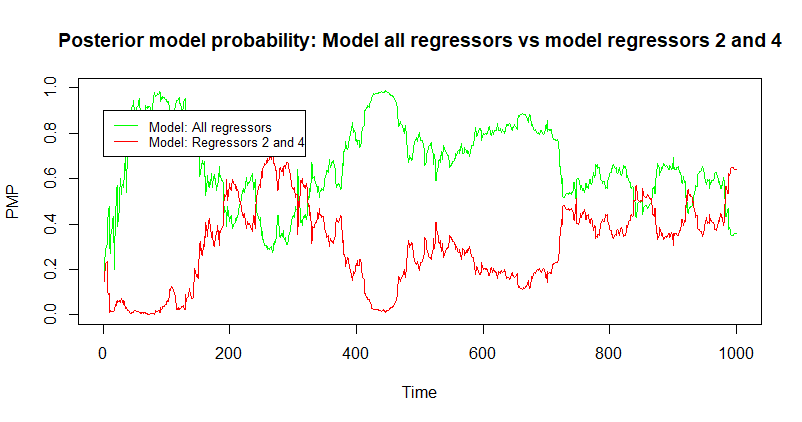
\includegraphics[width=340pt, height=200pt]{Chapters/chapter10/figures/dbmalogit.png}
	\caption[List of figure caption goes here]{Posterior model probability: Dynamic Bayesian model average, forgetting parameter equal to 0.99.}\label{figPMPdbma}
\end{figure}

\begin{figure}[!h]
	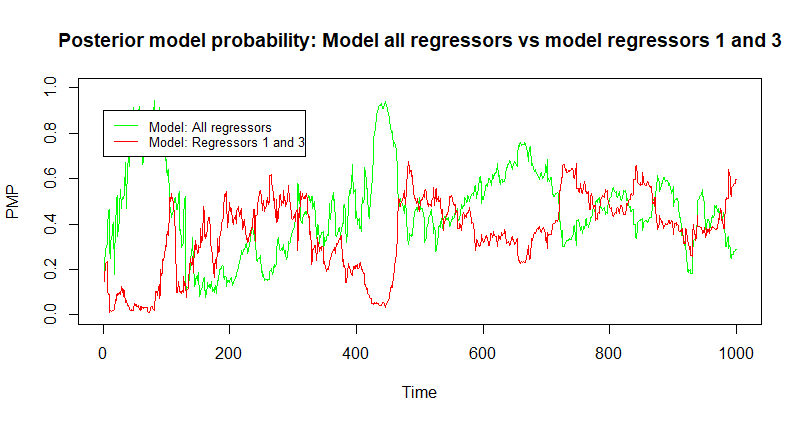
\includegraphics[width=340pt, height=200pt]{Chapters/chapter10/figures/dbmalogitN.png}
	\caption[List of figure caption goes here]{Posterior model probability: Dynamic Bayesian model average, forgetting parameter equal to 0.95.}\label{figPMPdbmaN}
\end{figure}

\item Show that 
\begin{align*}
	\mathbb{E}\left[\frac{p(\bm{\theta})}{\pi(\bm{\theta}|\mathcal{M}_m)p(\bm{y}|\bm{\theta}_m,\mathcal{M}_m)}\biggr\rvert \bm{y},\mathcal{M}_m\right]&=\frac{1}{p(\bm{y}|\mathcal{M}_m)},
\end{align*}
where the expected value is with respect to the posterior distribution given the model $\mathcal{M}_m$.

\textbf{Answer}

Given a probability density function $p(\bm{\theta})$, whose support is in $\bm{\Theta}$, then
{\footnotesize
\begin{align*}
	\mathbb{E}\left[\frac{p(\bm{\theta})}{\pi(\bm{\theta}|\mathcal{M}_m)p(\bm{y}|\bm{\theta}_m,\mathcal{M}_m)}\biggr\rvert \bm{y},\mathcal{M}_m\right]&=\int_{\bm{\Theta}}\left[\frac{p(\bm{\theta})}{\pi(\bm{\theta}|\mathcal{M}_m)p(\bm{y}|\bm{\theta}_m,\mathcal{M}_m)}\right]\pi(\bm{\theta}|\bm{y},\mathcal{M}_m)d\bm{\theta}\\
	&=\int_{\bm{\Theta}}\left[\frac{p(\bm{\theta})}{\pi(\bm{\theta}|\mathcal{M}_m)p(\bm{y}|\bm{\theta}_m,\mathcal{M}_m)}\right]\frac{\pi(\bm{\theta}|\mathcal{M}_m)p(\bm{y}|\bm{\theta}_m,\mathcal{M}_m)}{p(\bm{y}|\mathcal{M}_m)}d\bm{\theta}\\
	&=\frac{1}{p(\bm{y}|\mathcal{M}_m)}\int_{\bm{\Theta}}p(\bm{\theta})d\bm{\theta}\\
	&=\frac{1}{p(\bm{y}|\mathcal{M}_m)}.
\end{align*}
}
	
\end{enumerate}